\chapter{El microchip}\label{chapter:microchip}
Tiempo después \emph{Shockley} dejó los \emph{Laboratorios Bell}, y en la gala anual de la \emph
{Cámara de Comercio de Los Ángeles} donde fue galardonado por su invención, conoció a \emph{Arnold
Beckman} para el cual comenzó a trabajar en la división \emph{Laboratorio de semiconductores de Shockley}, 
parte de su empresa \emph{Beckman Instruments}, que se ubicó en \emph{Palo Alto}. En ese momento \emph{Shockley}
intentó reclutar a algunos de los investigadores que trabajaron con él en los \emph{Laboratorios Bell}, pero lo
conocían muy bien, su personalidad y su ego los espantaron. Por eso se dedicó a escribir una lista de los mejores
ingenieros de semiconductores del país. Sus más importantes contrataciones fueron \emph{Robert Noyce} doctor en 
física del \emph{Massachussets Institute of Technology}(\textbf{MIT}) y el químico \emph{Gordon Moore}. Con el paso 
del tiempo muchos de los expertos que contrató \emph{Shockley} se dieron cuenta de que era un líder incompetente, 
que cuando se equivocaba al tomar una decisión buscaba a alguien más a quien culpar, además, su indisposición a 
compartir el crédito le imposibilitó crear un espíritu de colaboración entre los hombres bajo su mando. De esta forma,
con el paso del tiempo la situación se hizo insostenible, hasta el punto que un grupo de trabajadores le dijeron a 
\emph{Arnold Beckman} que si \emph{Shockley} seguía, ellos renunciarían. Y así lo hicieron, ante la voluntad de \emph
{Beckman} de mantener a \emph{Shockley} a cargo de aquella división. Entre ellos estaban \emph{Robert Noyce} y \emph
{Gordon Moore}, y todos tenían el objetivo de crear una empresa que rivalizara con \emph{Beckman Instruments}. Para eso
eran necesarios fondos de los que no disponían, y luego de pasar mucho tiempo en búsqueda de una persona dispuesta a 
invertir en el negocio de los semiconductores, alguien sugirió ir a ver a \emph{Sherman Fairchild}, quien dispuso de
\$1.5 millones para la creación de la compañía, que se llamaría \emph{Fairchild Semiconductors}.\\
En un artículo escrito en conmemoración del décimo aniversario del \textbf{transistor}, publicado en 1957 justo
cuando se formó \emph{Fairchild Semiconductor} y el satélite ruso \emph {Sputnik} había sido lanzado, un ejecutivo
de los \emph{Laboratorios Bell} identificó un problema que apodado "la tiranía de los números". Como el número de
componentes en un circuito aumentó, el número de conexiones aumentó mucho más rápido. Si un sistema tenía, por
ejemplo, diez mil componentes, harían falta 100.000 o más pequeños enlaces de cables en las placas de circuitos,
la mayoría de las veces soldado a mano. Esta no era una receta acequible, sin embargo era una pieza fundamental
para un nuevo gran descubrimiento. La necesidad de resolver un problema que iba empeorando coincidió muchos pequeños
avances en formas para fabricar semiconductores. Esta combinación produjo un invento que ocurrió de forma independiente
en dos lugares diferentes, \emph{Texas Instruments} y \emph{Fairchild Semiconductor}. \brackcite{isaacson_2014}\\ 

\section{La primera solución}
\emph{Jack Kilby} era otro de esos chicos del Medio Oeste rural que jugueteaba en el taller con su padre y construía radioaficionados.
Durante una ventisca usaron un equipo radioaficionado para mantenerse en contacto con las áreas donde los clientes habían perdido el servicio
telefónico, y el joven \emph{Kilby} quedó fascinado por la importancia de tales tecnologías. “Fue durante una tormenta de hielo en mi
adolescencia", le dijo a \emph{T. R. Reid} del \emph{Washington Post}, "que vi por primera vez cómo la radio y, por extensión, la electrónica,
podrían tener un gran impacto en la vida de las personas manteniéndolos informados y conectados, y dándoles esperanza”. Luego de ser rechazado 
por el \textbf{MIT}, fue a estudiar a la universidad de \emph{Illinois}, pero lamentablemente sus estudios se vieron interrumpidos por la guerra 
luego de \emph{Pearl Harbor} y se unió a la marina de guerra. Era un tipo gentil con una amplia sonrisa. Lo que lo hacía especial era su
curiosidad insaciable sobre los inventos. Empezó a leer cada nueva patente emitida. "Tú lees todo, eso es parte del trabajo”, dijo. “Acumulas
todo este conocimiento, y esperas que algún día tal vez una millonésima parte sea útil”.\\
Su primer trabajo fue en \emph{Centralab}, una empresa de \emph{Milwaukee} que fabricaba piezas electrónicas. En este lugar se experimentó con
formas de combinar los componentes utilizados para fabricar audífonos sobre una sola base de cerámica, un precursor tosco de la idea para un \textbf
{microchip}. En 1952 \emph{Centralab} fue una de las empresas que pagó \$25,000 por una licencia para fabricar transistores, y fue el beneficiaria
de la voluntad de los \emph{Laboratorios Bell} de compartir su conocimiento. \emph{Kilby} asistió a un seminario de dos semanas en este lugar,
luego del cual se dió cuenta que para estar a la vanguardia en el desarrollo de los transistores necesitaba estar en una compañía más importante.\\
Por esta razón, luego de barajar varias opciones, en 1958 decide unirse a \emph{Texas Instruments}, donde se pondría a trabajar con \emph{Pat
Haggerty} y su brillante equipo de investigación de transistores dirigido por \emph{Willis Adcock}. Las primeras semanas trabajando allí \emph
{Kilby} se dedicó a experimenta que otra cosa podríá hacer con el \textbf{silicio}, además de convertirlo en transistores. Sabía que si creabas
un poco de \textbf{silicio} sin impurezas, actuaría como una simple \textbf{resistencia}. También se dió cuenta de que había una manera de hacer
que una \textbf{unión p-n} en una pieza de \textbf {silicio} actúe como un \textbf{capacitor}, lo que significa que podría almacenar una pequeña
carga eléctrica. De hecho, podrías hacer cualquier componente electrónico de \textbf{silicio} tratado de forma diferente. De eso el se le ocurrió
lo que se conoció como la “idea monolítica”: se podía hacer todos estos componentes en una pieza monolítica de \textbf{silicio}, eliminando la
necesidad de soldar juntos diferentes componentes en un circuito junta. \emph{Kilby} lo describió en su cuaderno de laboratorio en una oración
que luego sería citado en su mención del \emph {Premio Nobel}, "Los siguientes elementos del circuito podrían hacerse en una sola rebanada:
resistencias, condensador, condensador distribuido, \textbf{transistor}." Luego dibujó algunos bocetos toscos de cómo construir estos componentes
configurando secciones de silicio que habían sido dopadas con impurezas para tener diferentes propiedades en una sola losa. \brackcite{isaacson_2014}\\  

\begin{figure}[htb]
	\centering
	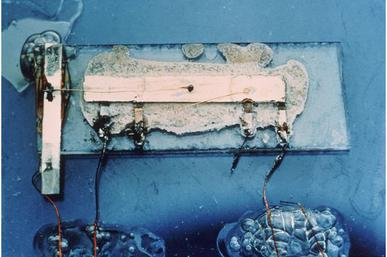
\includegraphics[scale = 0.8]{Graphics/kilby_first_microchip.jpg}
	\caption{Primer circuito integrado híbrido creado por \emph{Jack Kilby} utilizando \textbf{germanio}}
	\label{fig:7}
\end{figure}

\section{El enfoque de \emph{Noyce}}
\emph{Noyce} y sus colegas de \emph{Fairchild} habían estado buscando la posibilidad de un \textbf{microchip} desde enfoque. Comenzó cuando se vieron
golpeados por un problema complicado: sus transistores no funcionaban muy bien. Demasiados de ellos fallaban. Una pequeña cantidad de polvo
o incluso la exposición a algunos gases podía causar que dejaran de funcionar, también lo podía causar incluso un pequeño golpe. \emph{Jean Hoerni},
un físico de \emph{Fairchild} que fue uno de los ocho que abandonaron \emph{Beckman Instruments} a causa de \emph{Shockley}, se le ocurrió una solución
ingeniosa. En la superficie de un \textbf{transistor} de \textbf{silicio}, él colocaría una fina capa de óxido de \textbf{silicio}, como el glaseado
encima de un pastel de capas, que protegería el \textbf{silicio} de abajo. “La formación de una capa de óxido. . . en la superficie del \textbf{transistor}”,
escribió en su cuaderno, “protegerá las uniones expuestas de la contaminación.” El método se denominó "el proceso plano" debido al plano de óxido que se
sentó encima del \textbf{silicio}. En enero de 1959 (después de que \emph{Kilby} idear sus ideas pero antes de que fueran patentadas o anunciadas),
\emph{Hoerni} tuvo otra “epifanía” mientras se duchaba una mañana: minúsculas ventanas se pueden grabar en esta capa protectora de óxido para permitir
que las impurezas sean difundidas en puntos precisos para crear las propiedades deseadas de los \textbf{semiconductores}. \brackcite{isaacson_2014} \\ 

\begin{figure}[htb]
	\centering
	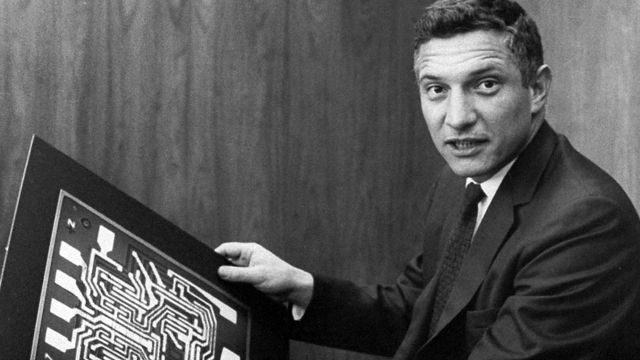
\includegraphics[scale = 0.8]{Graphics/Robert_Noyce_with_first_monolithic_IC_1959.png}
	\caption{\emph{Robert Noyce} con el primer circuito integrado (\textbf{microchip}) monolítico}
	\label{fig:8}
\end{figure}

\section{Una solución pacífica al tema de las patentes}
En 1959 ambas partes solicitaron patentes. \emph{Jack Kilby} y \emph{Texas Instruments} recibieron la patente de EE. UU. n.º 3.138.743 para \textbf{circuitos
electrónicos miniaturizados}. \emph{Robert Noyce} y \emph{Fairchild Semiconductor Corporation} recibieron la patente de EE. UU. n.º 2.981.877 para un \textbf
{circuito integrado} basado en \textbf{silicio}. En el verano de 1966, tres años antes de la resolución judicial final sobre a quien se le atribuiría el 
descubrimiento, \emph{Noyce} y sus abogados de \emph{Fairchild} se reunieron con el presidente y el consejo de \emph{Texas Instruments} y elaboraron un tratado
de paz. Cada empresa concedió que la otra tenía algunos derechos intelectuales y derechos de propiedad del \textbf{microchip}, y acordaron otorgar licencias
cruzadas a cualquier derecho que tuvieran. Otras empresas tendrían que hacer acuerdos de licencia con ambos, por lo general pagando una tarifa que ascendió
a aproximadamente 4 por ciento de sus ganancias. Las dos compañías sabiamente decidieron intercambiar licencias de sus tecnologías después de varios años de
batallas legales, creando un mercado global que ahora vale alrededor de \$ 1 billón al año. \brackcite{bellis_2017, isaacson_2014}\\ 

\section{Primeras aplicaciones}
Inicialmente, los \textbf{microchips} eran dispositivos estrictamente electrónicos. El éxito de los \textbf{microchips} ha llevado a la integración de otras tecnologías,
en un intento de obtener las mismas ventajas de pequeño tamaño y bajo costo. Estas tecnologías incluyen dispositivos mecánicos, ópticos y sensores. Los dispositivos de
carga acoplada y los sensores de píxeles activos estrechamente relacionados son chips que son sensibles a la luz. Han reemplazado en gran medida a la película fotográfica
en aplicaciones científicas, médicas y de consumo. Miles de millones de estos dispositivos ahora se producen cada año para aplicaciones, tabletas
y cámaras digitales. Los dispositivos mecánicos muy pequeños impulsados por electricidad pueden integrarse en chips, una tecnología conocida como sistemas microelectromecánicos.
Estos dispositivos se desarrollaron a fines de la década de 1980 y se utilizan en una variedad de aplicaciones comerciales y militares. Los ejemplos incluyen proyectores
DLP, impresoras de inyección de tinta y acelerómetros y giroscopios MEMS utilizados para desplegar las bolsas de aire de los automóviles. Desde principios de la década de 2000
, la integración de la funcionalidad óptica (computación óptica) en chips de \textbf{silicio} se ha buscado activamente tanto en la investigación académica como en la industria,
lo que resultó en la comercialización exitosa de transceptores ópticos integrados basados en \textbf{silicio} que combinan dispositivos ópticos (moduladores, detectores,
enrutamiento) con Electrónica basada en CMOS. También se están desarrollando circuitos fotónicos integrados que usan luz, utilizando el campo emergente de la física conocido
como fotónica. También se están desarrollando \textbf{microchip} para aplicaciones de sensores en implantes médicos u otros dispositivos bioelectrónicos. Deben aplicarse
técnicas de sellado especiales en dichos entornos biogénicos para evitar la corrosión o la biodegradación de los materiales semiconductores expuestos.\\
Los \textbf{microchips} se utilizan en muchos dispositivos electrónicos además de una computadora. En la década de 1960, la Fuerza Aérea usó \textbf{microchips}
para construir el misil Minuteman II. La \textbf {NASA} compró \textbf{microchips} para su proyecto \emph{Apolo}. Hoy en día, los \textbf{microchips} se utilizan
en los teléfonos inteligentes que permiten a las personas utilizar \emph{Internet} y tener una videoconferencia telefónica. Los \textbf{microchips} también se
utilizan en televisores, dispositivos de rastreo GPS, tarjetas de identificación y medicamentos. \brackcite{bellis_2021, wikipedia_2022_microchip}\\

\begin{figure}[htb]
	\centering
	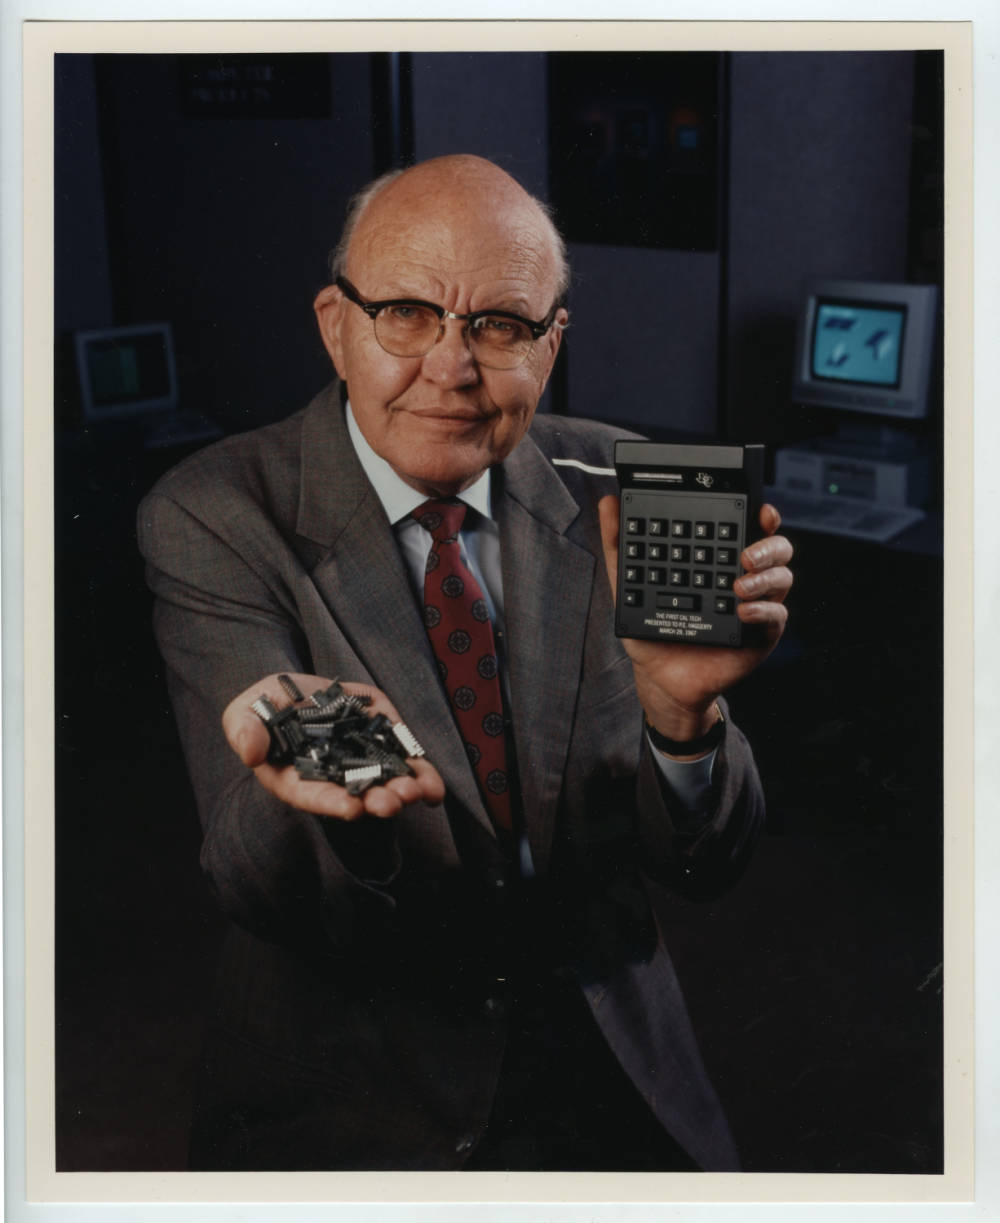
\includegraphics[scale = 2]{Graphics/Jack_Kilby_microchips_first_calculator.jpg}
	\caption{\emph{Jack Kilby} sosteniendo \textbf{microchips} y la primera calculadora presentada a \emph{Pat Haggerty} el 29 de marzo de 1967}
	\label{fig:9}
\end{figure}
